\section{Theoretische Grundlagen}
\subsection{Supraleiter}
Man nennt Materialien, deren elektrischer Widerstand unterhalb einer materialabhängigen kritischen Temperatur $T_{C}$ unmessbar klein wird, Supraleiter. Dabei verhalten sie sich wie ideale Diamagneten: Wird ein äußeres Magnetfeld angelegt, wird ein Strom in dem Supraleiter induziert, sodass im Inneren des Leiters ein Magnetfeld induziert wird, welches das äußere Feld genau kompensiert. Bei der Verdrängung Magnetfeldes aus dem Inneren des Supraleiters spricht man vom 'Meissner-Ochsenfeld-Effekt'.\\
Das Prinzip der Supraleitung basiert auf sogenannten 'Cooper-Paaren', makroskopischen Zuständen von zwei Elektronen, welche über hunderte Nanometer hinweg miteinander verbunden sind. Die Entstehung und Wirkung der Cooper-Paare wird durch die sogenannte 'BCS-Theorie' beschrieben, welche noch ausführlich diskutiert wird.\\
Es kann durch steigende Temperatur (für $T>T_{C}$), aber auch durch große externe Ströme, ein starkes äußeres Magnetfeld oder ein externes elektromagnetisches Wechselfeld der Größenordnung $\omega\approx \Delta E/\hbar$, mit welchem Elektronen über die 'Bandlücke' des Supraleiters angeregt werden, die Supraleitung unterbrochen werden.\\
~\\
Es werden zwei Arten von Supraleitern unterschieden:\\
\textbf{Typ I}\\
Das innere Magnetfeld sinkt unterhalb einer kritischen äußeren Magnetfeldstärke $H_{C}$ auf 0 (wenn $T<T_{C}$). Das Magnetfeld dringt  nur wenige Nanometer in den Leiter ein.\\
~\\
\textbf{Typ II}\\
Diese Art von Supraleiter wird auch 'Hochtemperatursupraleiter' genannt, da die kritischen Temperaturen deutlich höher sind als diejenigen für Supraleiter von Typ I. \\
Es werden zwei Stufen für das innere Magnetfeld unterschieden:  Unterhalb der externen Feldstärke $H_{C_{2}}$ sinkt die innere Feldstärke auf kleine Werte, unterhalb von $H_{C_{1}}$ auf null. Zwischen diesen beiden Feldstärken kommt es zur Bildung von Flussfäden im Leiter, welche lokal für einen kleinen Feldbeitrag sorgen. 
\subsection{BCS-Theorie}
Wie bereits erwähnt, wird die Supraleitung mittels Cooper-Paare, welche aus zwei Elektronen bestehen, die über hunderte Nanometer miteinander wechselwirken, durch die BCS-Theorie (benannt nach ihren Entwicklern John \textbf{B}ardeen, Leon N. \textbf{C}ooper und John R. \textbf{S}chrieffer) erklärt.\\
Die gegenseitige Anziehung der Elektronen beruht auf der Trägheit der positiv geladenen Atomrümpfe. Kommt es zu Gitterschwingungen im Kristall, so wandern die Atomrümpfe langsamer in ihre Ausgangsposition zurück als die Elektronen. Aus diesem Grund ziehen - bildlich gesprochen - Elektronen einen Schweif positiver Polarität hinter sich her. Dieser kann ein Elektron ähnlicher Energie und entgegengesetztem Spin anziehen, wodurch sich ein Cooper-Paar bildet. \\
Um möglichst viele solche Paare zu erhalten, muss eine tiefe Temperatur vorherrschen, damit alle Zustände bis zur Fermi-Energie gefüllt sind. Auf diese Weise gibt es viele Elektronen ähnlicher Energie und kaum thermische Anregung: Die schwache Wechselwirkung zwischen den beiden Elektronen, welche das Cooper-Paar formen, wird also nicht aufgebrochen. Die einzelnen Elektronen bilden nun nicht mehr Fermionen, sondern dank der Spinkopplung miteinander ein Boson. Die Wechselwirkungsenergie ist dabei kleiner als die der einzelnen Ladungsträger.\\
Da die Bosonen nicht dem Pauli-Prinzip unterliegen, können beliebig viele Cooper-Paare denselben Zustand, auch den Grundzustand, einnehmen. Dadurch kommt es zu keiner Wechselwirkung mit dem Rest des Leiters mehr, was der Grund für den unmessbar kleinen elektrischen Widerstand ist. \\
Kommt es zum Zusammenbrechen der Supraleitung, werden eigentlich die Cooper-Paare aufgebrochen. Bei dem Entstehen eines Cooper-Paares wird Energie frei. Wird diese Energie einem Cooper-Paar zugeführt, kann dieses aufgebrochen werden. Unterschiedliche Methoden hierfür wurden im Unterkapitel 'Supraleiter' beschrieben.
\subsection{Flussquantisierung}
Der in diesem Versuch verwendete Supraleiter hat die Form eines Ringes. Der magnetische Fluss kann somit mithilfe des Stoke'schen Satzes über das geschlossene Integral des Vektorfelds $\vec{A}$ über die Leiterschleife berechnet werden: 
\[\oint\vec{A}d\vec{l}=\Phi_{B}.\]
Da sich, wie bereits diskutiert, alle Cooper-Paare im gleichen Zustand befinden, können sie als Gesamtwelle betrachtet werden. Somit ist es klar, dass sich die Phase $\theta$ bei einem Umlauf nur um Vielfache von $2\pi$ ändern kann: 
\[\oint\triangledown\theta d\vec{l}=\Delta\theta=n\cdot 2\pi,\] 
wobei $n\in\mathbb{N}$.\\
Somit ergibt sich die Quantisierung des magnetischen Flusses im geschlossenen Supraleiter in sogenannten Flussquanten: 
\[\left|\Phi_{B}\right|=n\frac{\hbar}{2e}=n\Phi_{0},\]
wobei $\Phi_{0}=2,067833667\cdot10^{-15}Tm^{2}$ (Quelle: [ver]).
\subsection{Josephson-Effekt}
Der Josephson-Effekt tritt auf, wenn ein dünner Isolator ('Josephson-Kontakt') zwischen zwei Supraleiter gebracht wird.
\begin{figure}[h]
\begin{center}
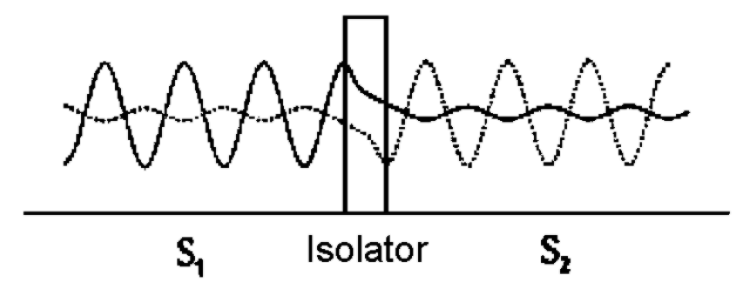
\includegraphics[scale=0.6]{Bilder/josephson}
\caption{Josephson-Kontakt zwischen zwei Supraleitern. Quelle: [ver].}
\end{center}
\end{figure}
~\\
Aufgrund der geringen Breite des Kontakts (wenige Nanometer) können Cooper-Paare mit hoher Wahrscheinlichkeit durch ihn tunneln, wodurch ein Tunnelstrom verursacht wird.\\
Wenn der Josephson-Kontakt, wie in diesem Experiment, zwischen zwei identischen Supraleitern ohne Potentialdifferenz liegt (dies ist hier der Fall wegen der Ringform des Supraleiters), so hängt der Tunnelstrom ausschließlich von der Phasendifferenz der einlaufenden Wellen ab. Der Josephson-Kontakt verhält sich zwar für den Strom wie ein schwacher Supraleiter, kann aber dennoch von einem äußeren Magnetfeld durchdrungen werden. Dadurch kann die Kopplung der Wellen und ihre Phasenlage verändert werden. \\
Solange sich das Material im supraleitenden Zustand befindet, fließt ein Gleichstrom von tunnelnden Cooper-Paaren, der 'Josephson-Gleichstrom' genannt wird. Wird aber eine kritische Stromstärke $I_{C}$ überschritten, so beginnen die Cooper-Paare aufzubrechen. \\
Der Tunnelstrom/'Josephson-Gleichstrom' kann in Abhängigkeit eines äußeren magnetischen Flusses $\Phi_{m}$ und dem Flussquant folgendermaßen geschrieben werden:
\[I=I_{0}\cdot\frac{sin(\pi\Phi/\Phi_{0})}{\pi\Phi/\Phi_{0}}.\] 
Der dazugehörige Graph sieht folgendermaßen aus:
\begin{figure}[h]
\begin{center}
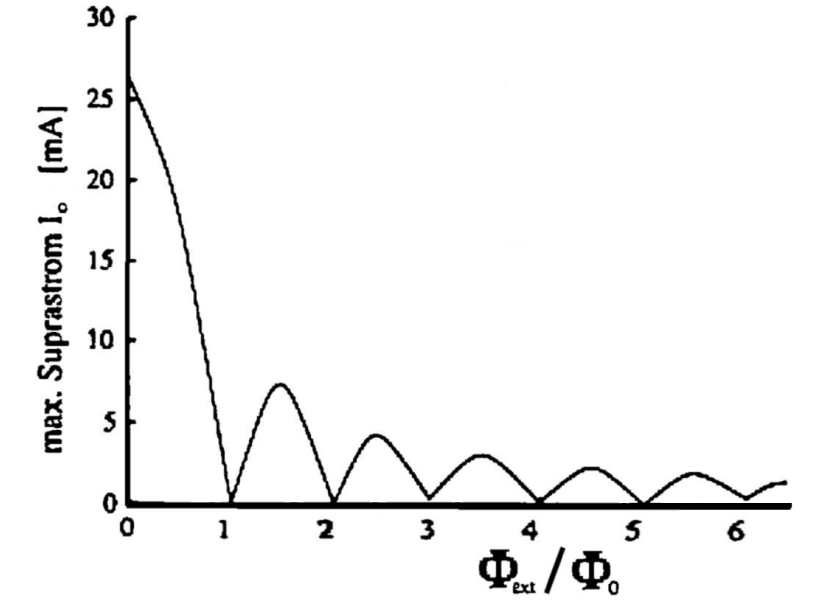
\includegraphics[scale=0.6]{Bilder/tstrom}
\caption{Maximaler Tunnelstrom durch den Josephson-Kontakt in Abhängigkeit des externen magnetischen Flusses. Quelle: [ver]}
\end{center}
\end{figure}